\section{Research Plan}

\subsection{Overview}

\begin{figure}[t]
\centering
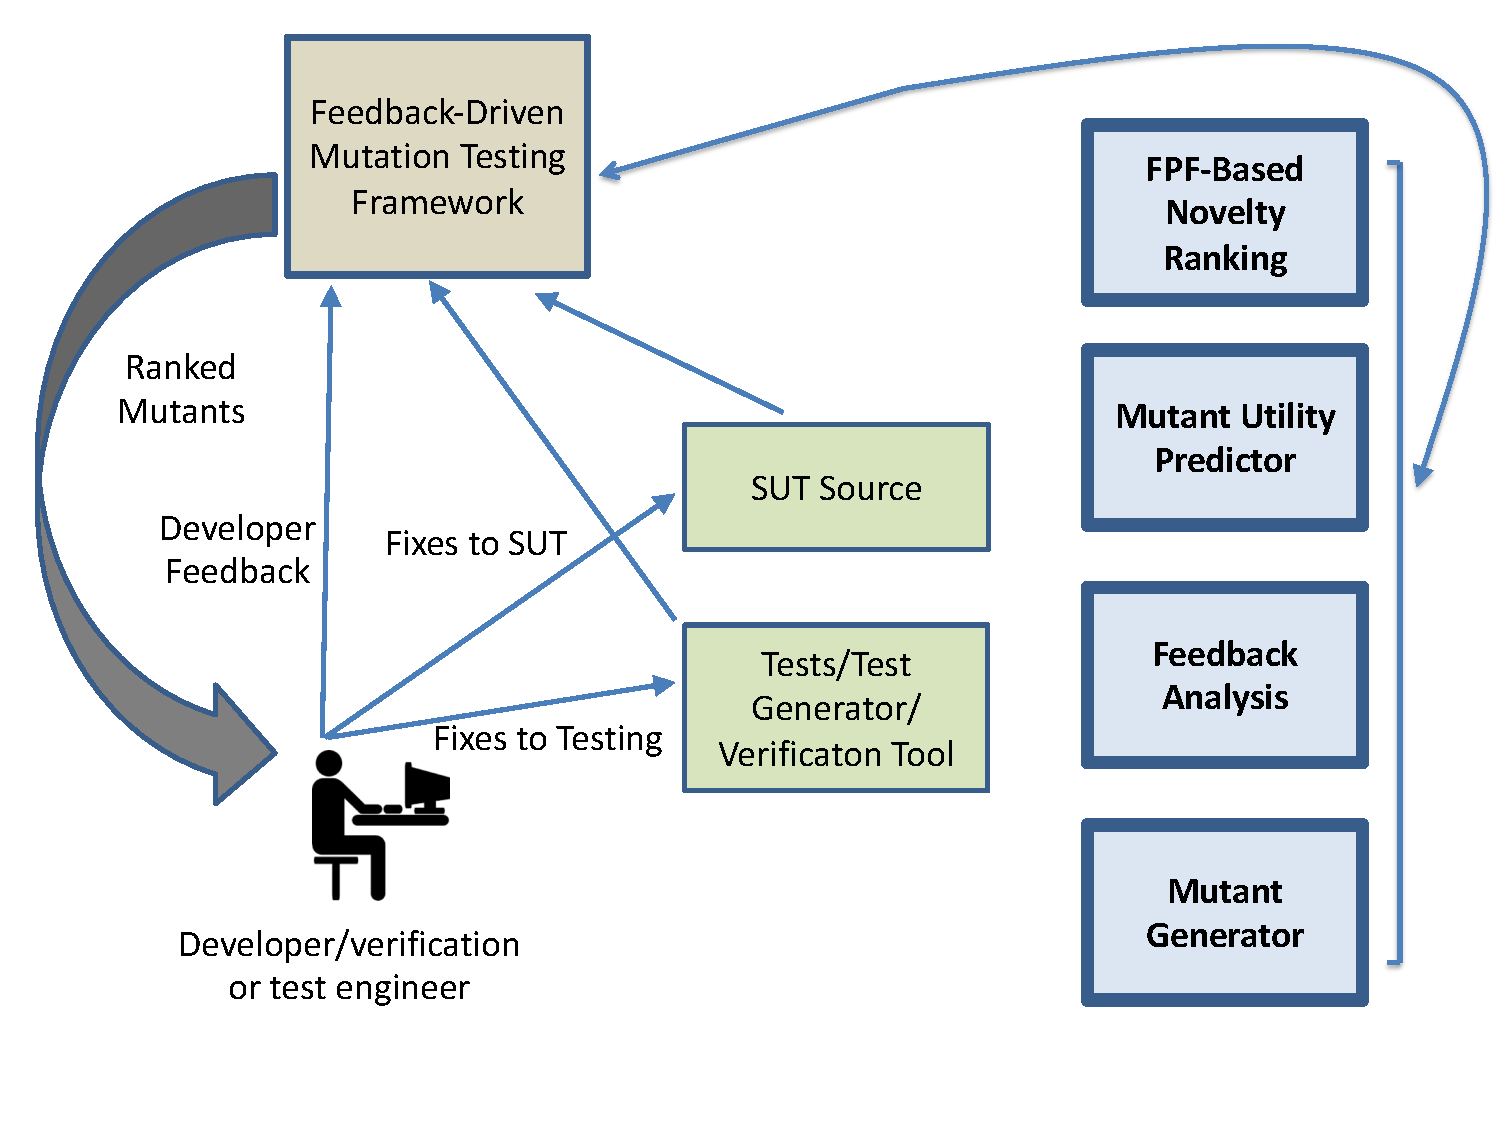
\includegraphics[width=0.8\columnwidth]{TestFlow}

\caption{Basic flow of feedback-driven mutation testing.}
\label{fig:flow}
\end{figure}

Figure \ref{fig:flow} shows the basic outline of a proposed workflow
and components needed to support feedback-driven mutation testing.
These components serve to organize the research plan.


\subsubsection{FPF-Based Novelty Ranking}
\label{sec:fpfplan}

\begin{figure}[t]
\centering
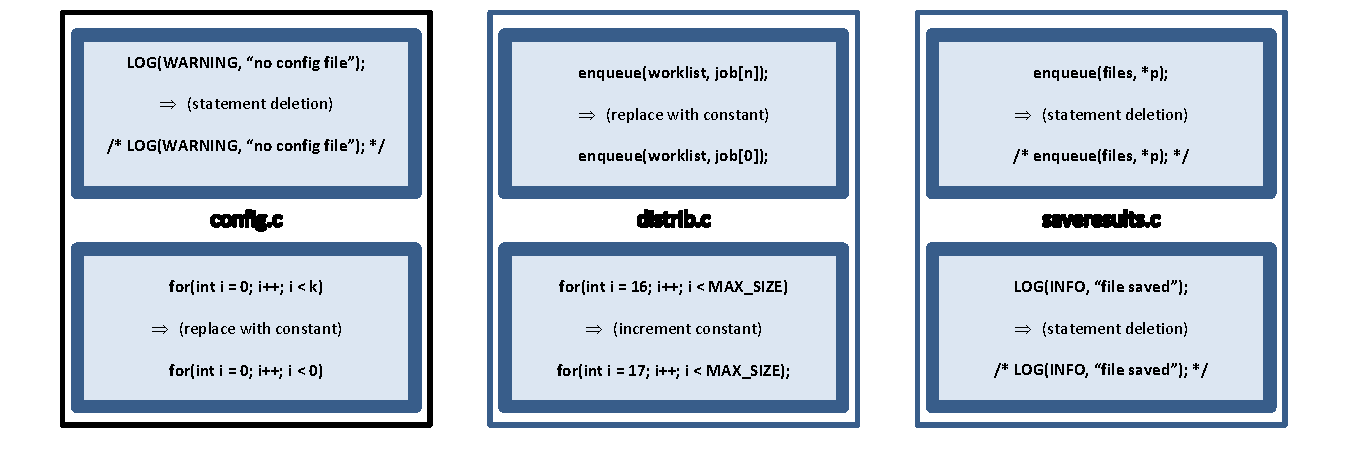
\includegraphics[width=0.95\columnwidth]{distmetric}

\caption{Which mutants are most similar?  If the user marked the
  mutant in the upper left corner as uninteresting and added a test
  to kill the
  mutant in the upper middle, which mutant
  should she examine next?}
\label{fig:distances}
\end{figure}

Ranking unkilled mutants according to how much ``new'' information they might
provide to users requires more than simply using the FPF algorithm as
in fuzzer taming.  The key difference is the problem of determining
how similar two mutants are; in fuzzer taming, it is possible to
extract a large amount of information about similarity of failing
tests from executing the tests, and, in fact, from executing the tests
on program mutants~\cite{PLDI13,distMut}.  There is no obvious equivalent
``run the mutant'' for mutants, and avoiding the expense of running
the test suite on uninteresting mutants is one of the goals of
feedback-driven mutation testing in the first place.

FPF requires a distance metric, and a distance metric requires a
\emph{representation} of mutants.  Mutants can be similar because they
modify the same line, function, class, or module, but also because,
despite being located in very different parts of a program, they are
very semantically similar.  E.g., a mutant to the parser of a compiler, to
an I/O error-handling routine in the code generator, and to a complex
optimization pass may all be very ``similar'' in the only meaningful
sense if all three mutants modify logging statements that don't have
any actual effect on the state of the compiler.  Figure
\ref{fig:distances} shows the fundamental problem.  It is not,
a-priori, obvious which mutants here are most (dis-)similar.  Every
mutant has multiple plausible ``nearest neighbors'' --- another mutant
in the same file (likely to impact the same aspects of correctness),
another mutant with very similar code (likely to have the same kind of
semantic impact on the local context), or another mutant with the same operator (perhaps
likely to have some similarity, though probably of a lower importance
than the previous two types of similarity.  Are all logging statements
equivalent, or are only {\tt INFO} logging calls similar, while every
{\tt WARNING}, {\tt ERROR} or {\tt FATAL} is unique?  Some of these
decisions are unlikely to be project-independent, and so a good metric
may well change during feedback-driven mutation testing, in response
to information from users (see Section \ref{sec:feedbackplan} below).

Elements of the
distance metric obviously include, at minimum, mutant location, mutation operator, and
some representation of the code element modified --- language
construct, functions called, variables modified, and so forth.  These
static aspects may also be augmented with user feedback (as noted
above), but also with dynamic information obtained during the process,
such as frequency with which tests cover the mutated
statements/modules, or the way the mutant changes the
program path from the unmutated code in tests.  In fact, there may
need to be two distance metrics:  one for selecting likely candidate
mutants to execute, that uses only static information and user
feedback, and one that uses dynamic results from compiling and testing
mutants to refine the notion of similarity for likely-novel mutants.
This is therefore a quite complex problem in representation and weighting of elements of a
representation, especially for a language- and
project- agnostic metric, perhaps one open to tuning via feedback
analysis.  We plan to exploit metric learning
methods~\cite{kulis2012metric}, but are aware that to avoid over-fitting
to even a set of good examples, the final metric may have to be largely
hand-tuned, and designed to incorporate feedback and dynamically
extracted information, which is not easily handled with learned metrics.  In part this is due to the difficulty of establishing
large amounts of ground truth data, and the expectation that
cross-project data will be less valuable than project-specific data
extracted during the process itself; although there are unsupervised
approaches to metric learning~\cite{scholkopf1998nonlinear,tipping1999probabilistic}, the most popular approaches require supervision.

\subsubsection{Mutant Utility Predictor}

Novelty with respect to previously analyzed mutants is not the only
important characteristic of a mutant.  Presenting a novel, but likely
equivalent mutant is often a waste of time, though some equivalent
mutants can be useful for identifying optimization opportunities or
refactorings.  Furthermore, of two similar mutants next to be presented,
it is better to present one that is higher in the mutant dominance
hierarchy (the one such that its tests will kill more other mutants).
There has been some initial work on predicting mutant quality
attributes and utility~\cite{MutQuality,FaRM}, including estimating how hard mutants
will be to kill, statically.  In addition to advancing the
state-of-the-art in that respect, feedback-driven mutation testing
also requires determining how to balance the need for novelty and the
predicted utility of a mutant.  For example, a utility-driven ranking
might suggest avoiding a highly novel mutant because it is likely
equivalent; however, it may be that labeling this mutant as equivalent
lets the FPF ranking avoid numerous other similar mutants --- e.g.,
postponing labeling a logging statement as equivalent may not be a
good idea.

\subsubsection{Feedback Analysis}
\label{sec:feedbackplan}

The ``feedback-driven'' aspect of feedback-driven mutation analysis
requires that information from the user be given high priority in the
process, a process with no clear equivalent in any previously proposed
mutation testing work.  The most straightforward example is that if a
user adds a test to kill a mutant, and marks that as a ``high impact''
action (the omitted testing was potentially allowing serious faults to
pass without detection) or even ``fault-revealing'' (the new test
detected a real fault in the system), then it may be most effective to
abandon the search for novelty and instead search for very similar
mutants still not killed by any test, in the expectation that these
may also result in high impact or fault-revealing tests.  If a user
marks a mutant as ``equivalent, but indicative of a refactoring
opportunity'', the same logic may apply:  similar mutants in other
parts of the code base may show the same problem with code quality,
even if they are predicted to be equivalent, and are not highly
novel.  In addition to informing the system of how useful various
analyzed mutants were, a user should also be able to inform the system
about correct and incorrect novelty rankings:  if the system presents
a mutant that is, from the user's POV, a (near-)duplicate of an
already handled mutant, the user should be able to express this fact,
and avoid future similar bad novelty estimates.

\subsubsection{Mutant Generator}
\label{sec:anylangplan}

The source of all mutants to be presented to the user is the mutant
generator, and in order to maximize the effectivenes of the approach,
this proposal aims to allow effective generation of mutants for any
programming 
language or DSL, with minimal additional effort.  The {\tt
  universalmutator} provides an initial source of mutants that
satisfies this requirement for initial experimentation, but for
long-term effectiveness is both inefficient and inexpressive.  The
current implementation avoid parsing to such an extent that it
generates numerous useless mutants embedded in code comments, or that
are obviously syntactically invalid.  While avoiding a parser-based
approach, simple additonal constraints could avoid this, without
adding burden on users, such as allowing the definition of a
language's comment mechanisms, and not producing mutants inside
comments.  More generally, a mechanism for disabling mutation in
contexts defined in the same way as mutation operators would handle
other, even project-specific, constraints (e.g., never mutate inline
assembly in C/C++).  A problem with the current representation of
mutation operators and such contexts is that regular expressions are
currently applied only at the line level, and in any case are not
effective for defining such fundamentally non-regular aspects of code
as blocks and nested delimiters.  A key goal in this project is to
enhance the regular-expression language (without losing its simplicity
for ``normal'' operators) with the ability to express, in a
language-independent, syntactic form, such context-dependent aspects
of code; the Cobra code-checking tool's language~\cite{Cobra} is an
example of the kind of approach desired, though the language itself
must be different, since transformation,
not just detection, is the expressive content of a mutation operator.
Moreover, the generator will also need to be improved to allow users
to easily specify novel build environments and plugins for checking
Trivial Compiler Equivalence~\cite{TCE} to make the entire feedback-driven
mutation process workable.  To some extent, an efficient mutation
generator needs to incorporate aspects of mutation execution and even
post-mortem analysis of the results of a mutant.  Finally, for
extremely large projects, simply generating and storing all mutants
may be inefficient, and rather than processing the entire source code
and applying all mutation rules, a demand-driven mode that only
produces new mutants likely to be novel and of high utility may be required.

\subsection{Core Research Questions}

The component-focuses sections above provide an overview of the
research problems to be addressed by this proposal, but it is also
useful to consider the high-level research questions to be addressed,
some of which are cross-cutting concerns independent of any single
component, but potentially important to the development of a
practical, maximally efficient, feedback-driven mutation approach.

\subsubsection{Research Questions for Feedback-Driven Mutation Testing
in General}

\begin{enumerate}
\item What is a good generalized, language-agnostic representation
  of and distance metric for program mutants for use in FPF?
\item How can FPF-based selection of mutants for novelty best incorprorate
  predictions of mutant equivalence, outcome, dominance, and
  productivity?  Is novelty or expected utility more important?
\item How should feedback-driven mutation testing actually incorporate feedback from users into the 
  ranking of mutants? 
\item Is it possible to identify outliers in otherwise similar groups of
  mutants, and is such identification useful?
\item How should budgets for automated test generation and
  timeouts for verification efforts be chosen so as to quickly estimate whether a
  mutant is killable?
\item Is it possible to predict whether a mutant's unkillability is due to poor test 
  generation  or due to oracle weakness? 
\item How can feedback-driven mutation testing most effectively use already generated killing tests
  and counterexamples to prune mutants?
\item Is distance-based clustering plus timing information useful for quickly
  eliminating killable mutants similar to already-killed mutants?  How
  does this relate to Predictive Mutation Testing (PMT)?

\end{enumerate}

\subsubsection{Research Questions Specific to Any-Language Mutation}

\begin{enumerate}
\item What advances are required in order to maximize the efficiency and usability of a
  fundamentally language-agnostic regular-expression-based approach to
  mutant generation?
\item How should the language of regular expressions be extended to allow
  for language-agnostic definition of mutation operators that require
  more parser-like analysis of code structure, without compromising
  the usability and simplicity of the approach?
\item Is it possible to perform on-the-fly mutant generation for very
  large projects, and reconcile this approach with FPF (e.g., generate
  new mutants with, possibly approximate, desired distances from
  already evaluated mutants)?
\end{enumerate}

\subsection{Work and Evaluation Plans}
\label{sec:workplan}
\subsection{Evaluation Plan}
